\chapter{Using LaTeX to make documents that meet NREL's requirements}

A LaTeX class called \emph{nrel.cls} has been written that implements NREL's formatting requirements in LaTeX. Authors are required to use this class file to create NREL documents.

\section{NREL's LaTeX Environment}
\subsection{Web Interface}
NREL authors are strongly encouraged to use the NREL-hosted web-based latex environment. This can be found at \href{latex.nrel.gov}{latex.nrel.gov} and is based on the sharelatex web interface.

\subsection{Starting new documents}
\begin{enumerate}
\item Go to \href{https://github.com/NREL/latex_editing}{https://github.com/NREL/latex\_editing} and download the repository as a .zip file from the icon on the lower right hand side of the page.
\item Got to \href{latex.nrel.gov}{latex.nrel.gov} and start a new project by uploading the zip file. Modify the project properties (name, collaborators, etc) as required.
\item Modify \emph{main.tex} as required.
\end{enumerate}

\subsection{Working with pubhub}
pubhub is NREL's publications management software. All files used to prepare the latex document should be downloaded from \href{latex.nrel.gov}{latex.nrel.gov} and stored in pubhub once the final document has been published.

\section{The nrel.cls class file}\label{sec:nrelcls}
\emph{nrel.cls} provides the \emph{nrel} document style and controls the formatting and presentation of documents so that they meet NREL's requirements.

The \emph{nrel} document class is a meta-class, in that documents must also be identified as being one of the basic \LaTeX\ document classes in the options that are passed to the class. Options are passed to the class in the \verb+\documentclass+ line:

\begin{lstlisting}
\documentclass[option1,...,optionn]{nrel}
\end{lstlisting}

This line specifies the options (inside the square brackets) that will be passed to the \emph{nrel} class. The options include:
\begin{description}
\item[book]{compile the document using the LaTeX \emph{book} class. This is intended for longer documents and allows the use of chapters.}
\item[report]{compile the document using the LaTeX \emph{report} class. This is intended for longer documents and allows the use of chapters.}
\item[article]{compile the document using the LaTeX \emph{article} class. This is intended for shorter documents such as journal articles. This class does not support the use of chapters. The Github repository includes an example of the article option being passed to the NREL class in \emph{mainArticle.tex}.}
\item[memoir]{compile the document using the LaTeX \emph{memoir} class. This option is not recommended because of the challenge with later converting to RTF format for communications review.}
\item[draft]{add a `draft' watermark to all pages and colours all links in blue.}
\item[10pt, 12pt]{set the font size accordingly. The default is 12 point.}
\item[letterpaper, a4paper]{set the paper size. the default is letter paper.}
%\item[tagged]{create a tagged PDF}
\end{description}

\emph{nrel.cls} calls a variety of other packages. Packages are codes that modify the appearance or behaviour of LaTeX to achieve something. Table \ref{Tab:Packages} lists the packages that are explicitly called by \emph{nrel.cls} in the order they are called in. These packages often call other packages, so this is not an exhaustive list.

\begin{table}[!h]
\centering
\caption[Packages supported by the nrel.cls class]{Packages supported by nrel.cls.}
\label{Tab:Packages}
\begin{tabular*}{\textwidth}{llp{0.5\textwidth}}
\toprule
Packages & options & functionality\\
\midrule
%accessibility & tagged & generates the document structure and tagging \\
amsfonts, amssymb & & supplies AMS fonts, which are useful for mathematics \\
babel & english & \\
booktabs & & \\
caption & & \\
courier& & changes fonts \\
fontenc & T1 & \\
geometry & & sets page size and margins \\
graphicx & & graphics handling, including \emph{.eps} figures \\
helvet& & changes fonts \\
hyphenat & & \\
listings & & \\
mathptmx& & changes fonts \\
nag & & checks that packages are up to date and looks for bad habits in LaTeX code. \\
parskip & & \\
pdfcomment & & tool-tips. Also calls the \texttt{hyperref} package  \\
setspace & & \\
subfigure & & provides the \texttt{subfigure} environment to produce sub figures \\
toclof & subfigure & \\
toclifbind & nottoc, notlot, notlof & \\
todonotes & & inline and margin to-do notes \\
xcolor & & \\
\bottomrule
\end{tabular*}
\end{table}

\section{Creating Content}
\subsection{Front, main, and back matter}
NREL's convention is to have Roman numerals in the front matter, and then arabic numerals in the main matter of the document (after the tables of contents, figures and tables). Tables and figures in the front matter are also numbered differently (Table A, B, C, ...) than in the main matter (Table 1, 2, 3, ...).

This change in page and float numbering is implemented using the \verb+\frontmatter+, \verb+\mainmatter+, and \verb+\backmatter+ commands at the start of these sections of the document:

\begin{lstlisting}
\begin{document}

\maketitle
\frontmatter
...
\tableofcontents
\clearpage
\listoffigures
\listoftables
\mainmatter
...
\backmatter
\end{document}
\end{lstlisting}

Page numbering in the front matter (i.e. the Abstract, Summary, and Foreword chapters or sections) starts at page 3 to allow for NREL cover pages.

If you don't use the \verb+\frontmatter+ commands, you may need to increment the page counter manually. To increment the counter $n$ pages, use \verb+\setcounter{page}{n}+ after \verb+\begin{document}+.

\subsection{Cross references}
Use labels and references to refer back and forth to figures, equations, tables and sections. 

For example, an equation can be added using the following text:

\begin{lstlisting}
\begin{equation}
y = mx+c
\label{eqn:line}
\end{equation}
\end{lstlisting}

This gives the following:
\begin{equation}
y = mx+c
\label{eqn:line}
\end{equation}

And using the text \verb+Eqn. \ref{eqn:line}+ provides a cross reference to Eqn. \ref{eqn:line}.

\subsection{Floats}
Floats are images, tables or other pieces of the document that are free to move to the best place in the document for them. The two most common floats are the tabular environment (for tables) and the figure environment for figures.

\subsubsection{Tables}
Use the \texttt{tabular} environment to produce basic tables. Table~\ref{tab:widgets} is produced using this code: 

\begin{lstlisting}
\begin{table}[!h]
\centering
\caption{An example table.}\label{tab:widgets}
\begin{tabular}{lr}
Item & Quantity \\
\hline
Widgets & 42 \\
Gadgets & 13
\end{tabular}
\end{table}
\end{lstlisting}

\begin{table}[!h]
\centering
\caption{An example table.}\label{tab:widgets}
\begin{tabular}{lr}
Item & Quantity \\
\hline
Widgets & 42 \\
Gadgets & 13
\end{tabular}
\end{table}

Resist the temptation to stop table rows early. If all of the delimiters (\&) are included in each row, the table will be complete and will produce a better PDF.

\subsubsection{Figures}
To include a figure in a document, use the \texttt{figure} environment and the \texttt{includegraphics} command.

\begin{lstlisting}
\begin{figure}
\includegraphics[width=\textwidth]{figure's-file-name}
\caption{Caption goes here.}\label{fig:figuresLabel}
\end{figure}
\end{lstlisting}

\subsubsection{Subfigures}

Subfigures are implemented using the \texttt{subfig} package. The example below generates Figure \ref{fig:NRELimages}.

\begin{lstlisting}
\begin{figure}
\centering
\hfill
\subfigure[Wind turbines at the Forward Wind Energy Center in Fond du Lac and Dodge Counties, Wisconsin. (Photo by Ruth Baranowski / NREL) \label{fig:21206}]{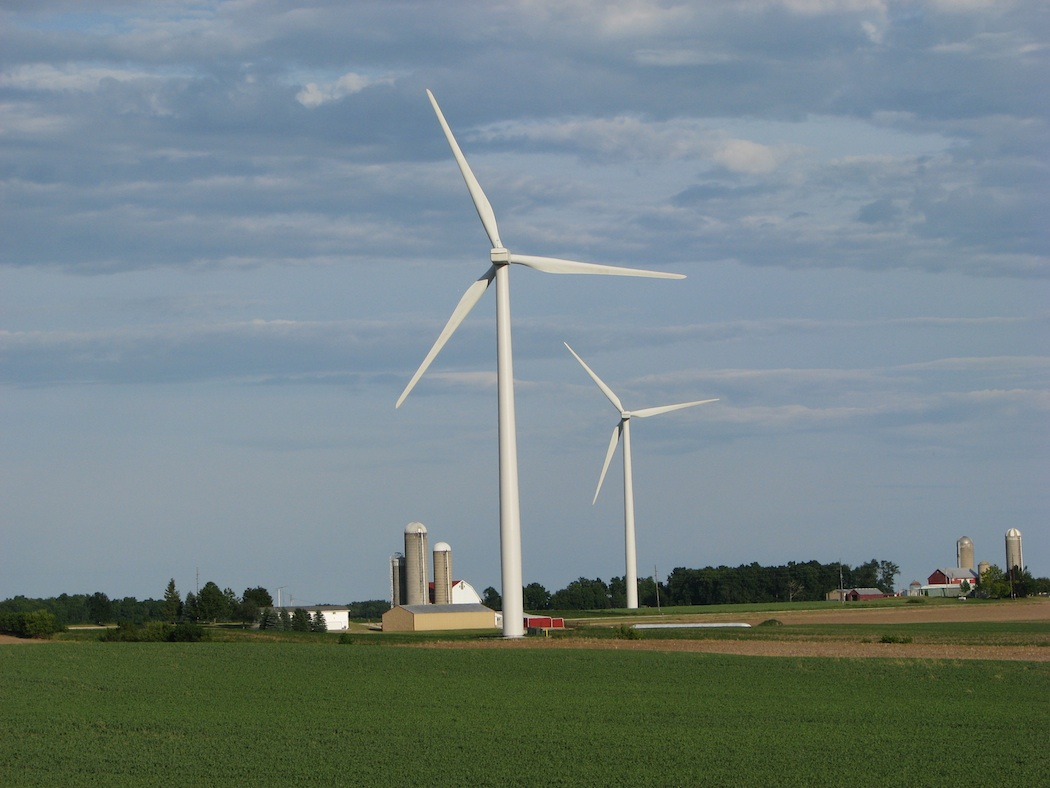
\includegraphics[height=2.5in]{files/21206}}
~
\hfill 
\subfigure[Aerial view of the National Wind Technology Center. (Photo by Dennis Schroeder / NREL)\label{fig:20018}]
 {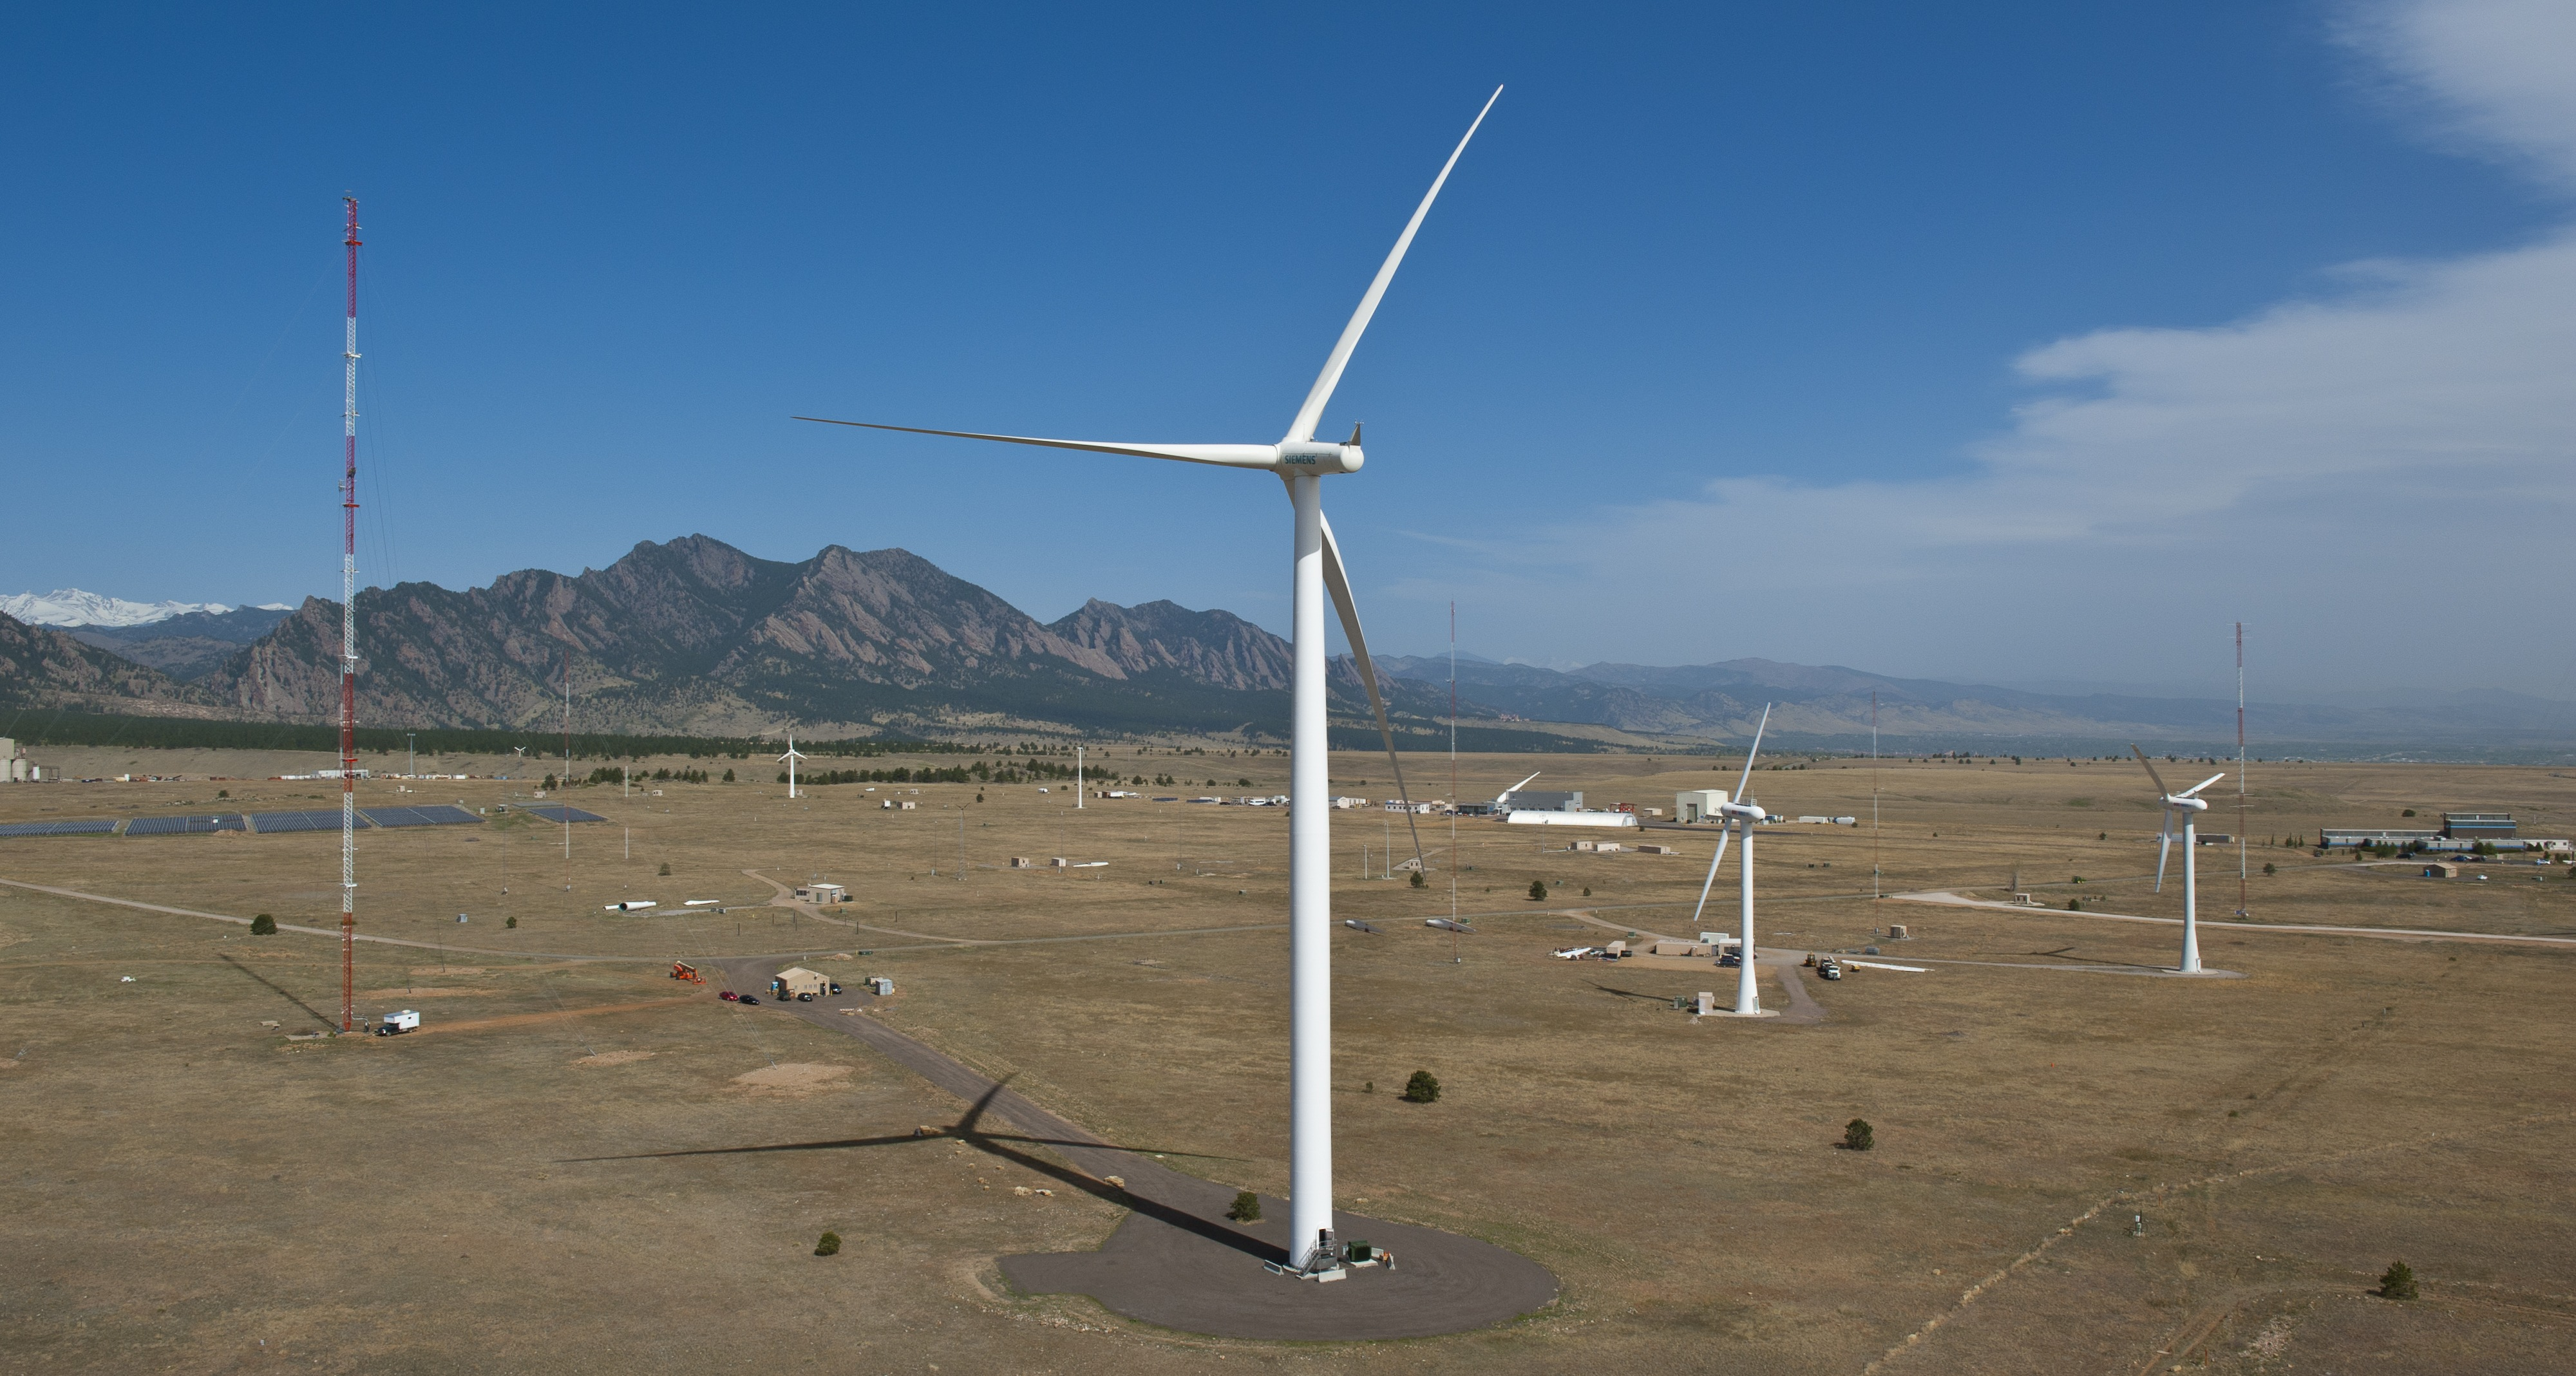
\includegraphics[height=2.5in]{files/20018}}
\hfill
\caption{NREL images}\label{fig:NRELimages}
\end{figure}
\end{lstlisting}
 
\begin{figure*}[htp]
\centering
\hfill
\subfigure[Wind turbines at the Forward Wind Energy Center in Fond du Lac and Dodge Counties, Wisconsin. (Photo by Ruth Baranowski / NREL)\label{fig:21206}]{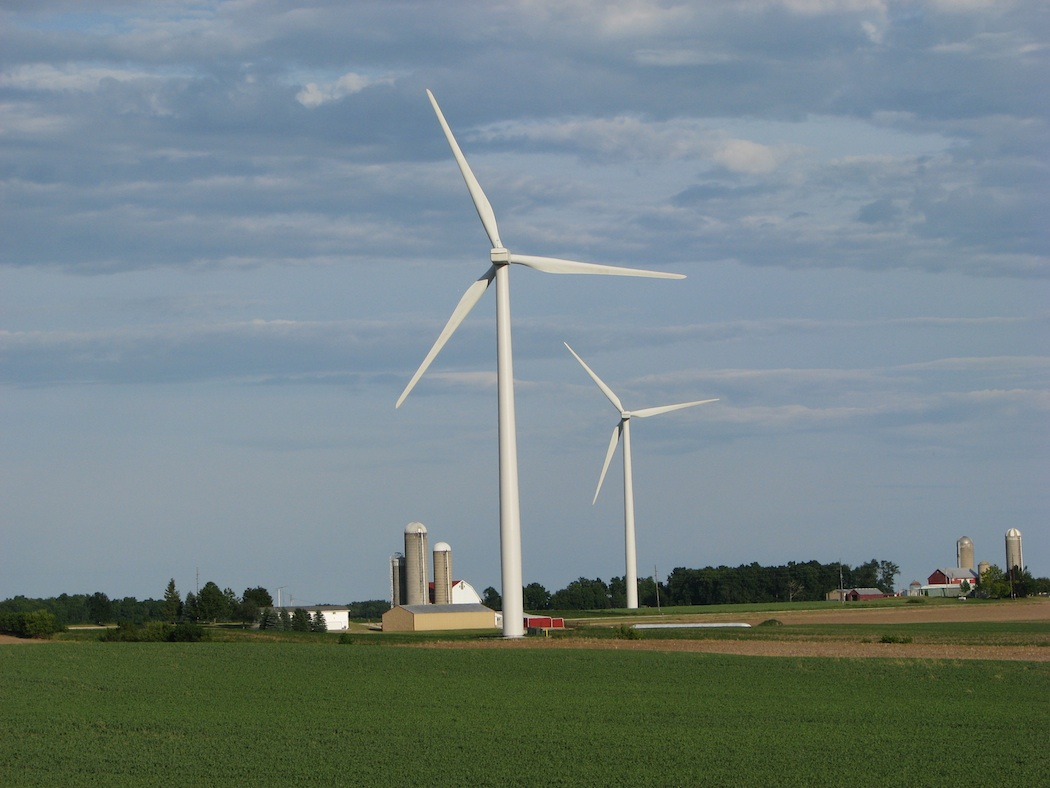
\includegraphics[height=2.5in]{files/21206}}
~ 
\hfill
\subfigure[Aerial view of the National Wind Technology Center. (Photo by Dennis Schroeder / NREL)\label{fig:20018}]{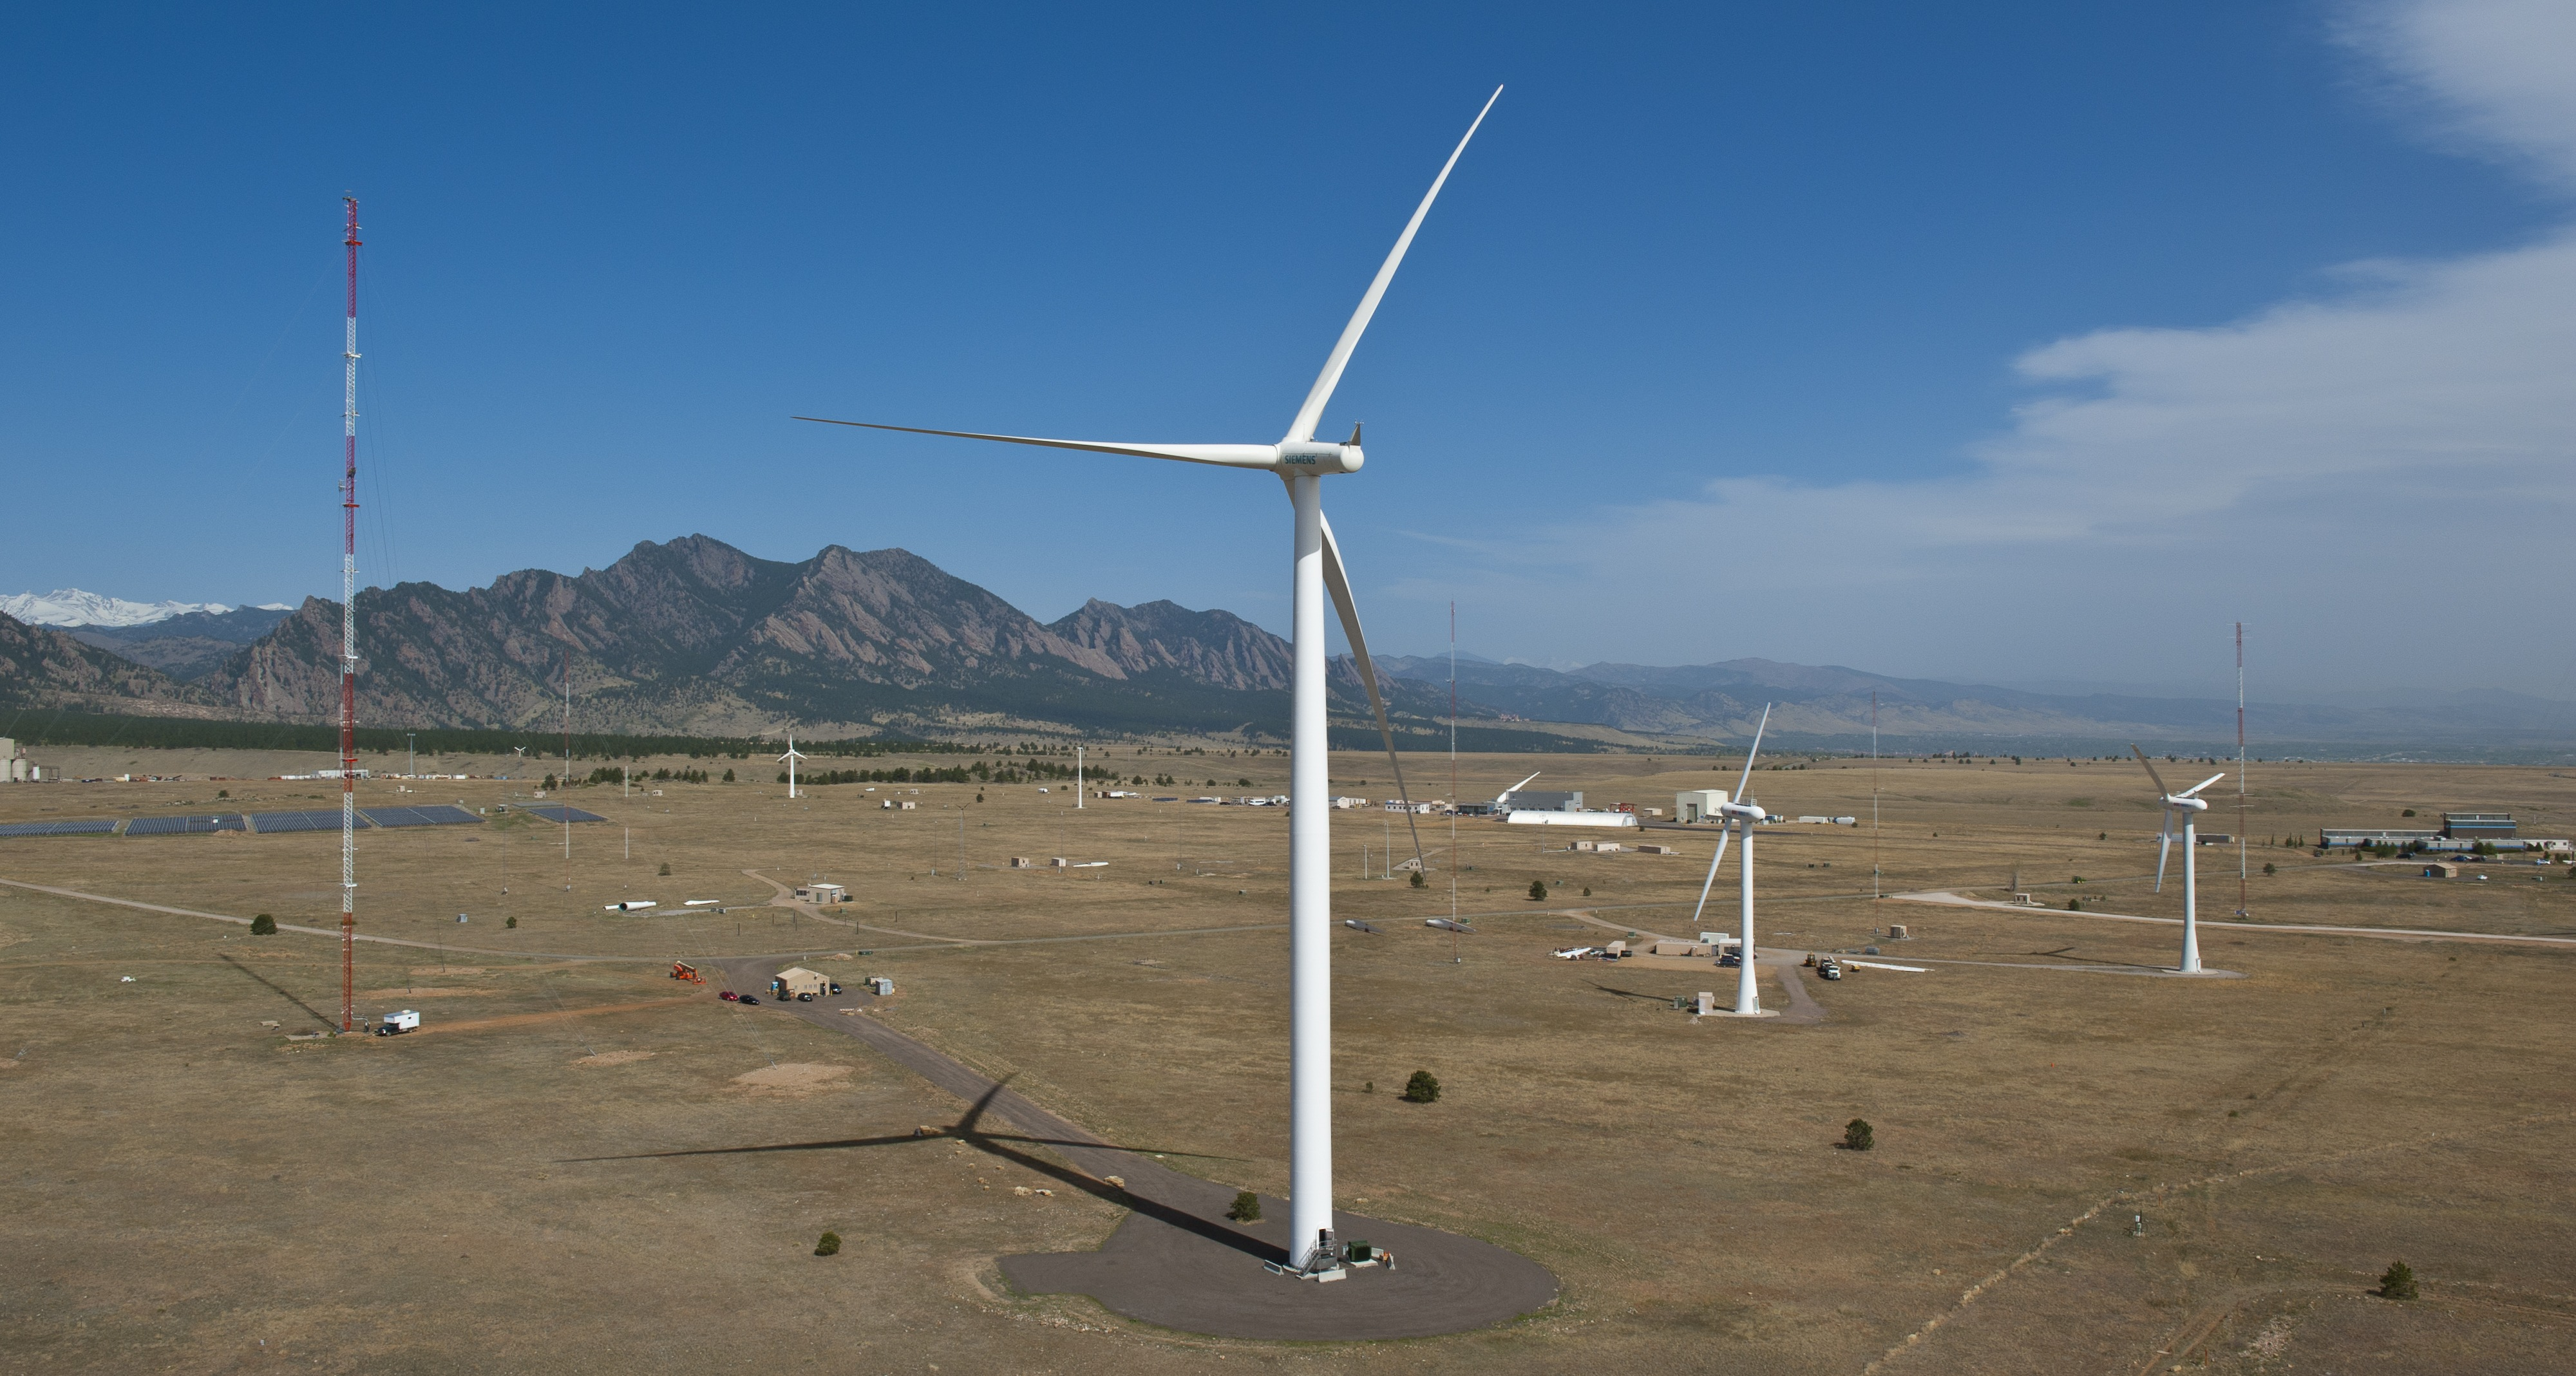
\includegraphics[height=2.5in]{files/20018}}
\hfill
\caption{NREL images}\label{fig:NRELimages}
\end{figure*}

\subsection{Citations}
\label{Sec:Bib}
Use \texttt{bibtex} to organize references and store them in a single file (e.g. \verb+/Documents/bibliography/bibliography.bib+). The bibliography will then contain entries with `keys' for each source, like \texttt{Lamport\_1986\_a}. 

Authors can then insert citations to this key throughout their document, using different styles of citation. Citations are generated using the \texttt{biblatex} package, which also formats references in the correct style.  Ways to generate citations are described in the \texttt{biblatex} documentation, and include:
\begin{itemize}
\item \verb+\cite{Lamport_1986_a}+ prints \cite{Lamport_1986_a}.
\item \verb+\citep{Lamport_1986_a}+ prints \citep{Lamport_1986_a}.
\item \verb+\citet{Lamport_1986_a}+ prints \citet{Lamport_1986_a}.
\end{itemize}

To cite URLs, use the 'misc' style. For example, the bibtex entry for \href{http://tex.stackexchange.com}{http://tex.stackexchange.com}\ \cite{texstackexchange} looks like this:

\begin{lstlisting}
@misc{texstackexchange,
	Author = {Anon.},
	Howpublished = {Accessed July 21, 2014: \url{http://tex.stackexchange.com}},
	Title = {\TeX -- LaTeX Stack Exchange},
	Year = {2014}}
\end{lstlisting}

This format will allow you to include the date on which a URL was accessed.

The citations should work with journal articles, books \citep{Lamport_1986_a}, technical reports \citep{TechReportTest}, and URLs \citep{texstackexchange}.

\subsection{Including computer code}
The \texttt{lstlisting} package has been loaded. 

To change the syntax highlighting use \verb+\lstset{language=[dialect]language,columns=fullflexible,keepspaces=true}+ before each listing where the language changes. For more details see the \texttt{lstlisting} documentation.

\subsection{NREL-style bibliographies}
NREL uses "Chicago A" style-references. The \emph{nrel.cls} file uses Biblatex to produce these references automatically. 

To include a bibliography in the document give the bibliography file location in the preamble, and insert the bibliography at the appropriate location:

\begin{lstlisting}
% give the bibliography file location
\bibliography{files/bibliography.bib}
...
\begin{document}
...
% insert the bibliography into the document
\cleardoublepage
\label{sec:Bib}
\printbibliography
...
\end{document}
\end{lstlisting}

\section{Creating a file structure}
\label{sec:FileStructure}
Your main file should be called \emph{main.tex}. This helps editors and coauthors identify where to start. Then, use \texttt{input} to import other files into your main file at compilation.

For example, each of the chapters in this report is in separate files, called \emph{WhatIsLatex} (Chapter 1), \emph{NRELRequirements.tex} (Chapter 2), \emph{LatexAtNREL.tex} (Chapter 3), and so-on. In the example available on Github, they are stored in the \emph{files} directory. \emph{main.tex} then looks like this:

\begin{lstlisting}
...
\begin{document}
% content
\chapter{What is LaTeX?}
LaTeX is a mark-up language that describes how a document should be prepared. Three things are needed to make a LaTeX document:
\begin{enumerate}
\item A source document, usually with extension \emph{.tex}
\item Some packages and classes that help turn what's in the source document into something helpful
\item A compiler, also referred to as a working LaTeX installation.
\end{enumerate}

At first glance the source document looks like a programming language, and that's because it is: LaTeX is not WYSIWYG, like many of the document preparation tools in common use today. A good analogy is html.

\section{Printed Resources}


\section{Online Resources}
The wikibook at \href{http://en.wikibooks.org/wiki/LaTeX}{http://en.wikibooks.org/wiki/LaTeX} is an excellent resource. There are also several internet forums such as \href{tex.stackexchange.com}{tex.stackexchange.com} that may be useful.

Documentation for the packages used in the nrel.cls file (Section \ref{sec:nrelcls}) can be found at \href{ctan.org}{ctan.org}.

\input{files/NRELRequirements}
\input{files/LatexAtNREL}
...
\end{lstlisting}

\section{Best practice in writing a document in LaTeX}
\begin{description}
\item[Create a structure before you get too far.] Authors will find it easier to write documents and make changes if they separate the content of the document from the structure.
\begin{enumerate}
\item Each new LaTeX document should be placed in it's own directory. 
\item Create a main LaTeX file that just contains the preamble, custom commands and uses \texttt{input} to call the content. See Section \ref{sec:FileStructure} for an example where each \texttt{chapter} is contained in its own file. In an article, each \texttt{section} could be contained in its own file.
\item Keep the number of packages used to a minimum. If authors feel that something is desperately missing, they can contact the maintainers of the \emph{nrel.cls} file. Not all packages can be used as they lack compatibility.
\end{enumerate}
\item[Focus on content, not appearance.] Don't spend hours trying to adjust fonts, headers or spacing between lines. 
\begin{enumerate}
\item The document produced should meet NREL's requirements if it is compiled using \emph{nrel.cls}. 
\item Don't throw in lots of \texttt{clearpage}s or other commands to push material around. LaTeX is designed to handle that. 
\item Resist the temptation to add or subtract space, change lengths or do other things to modify the layout. 
\item Write!
\end{enumerate}
\end{description}
